\section{共轭梯度法}
\label{sec:ls-conjugate-gradient}

设$\bm A=\bm A^\top\succ0$。\term{共轭梯度法}（conjugate gradient method，CG）在第$k$步取$\bm x_0+\mathcal K_k$中使误差的能量范数
\[
 \lVert\bm x-\bm x_\star\rVert_{\bm A}=\bigl((\bm x-\bm x_\star)^\top\bm A(\bm x-\bm x_\star)\bigr)^{1/2}
\]
最小的近似，这等价于第~\ref{sec:ls-krylov-selection-criteria}节的Galerkin条件。

它紧接第~\ref{sec:ls-lanczos-application}节的应用：那里在Lanczos基下把Galerkin条件化成了三对角方程，CG就是对称正定时求解这个方程的一种特殊做法。

\subsection{主要思想}
\label{sec:ls-cg-derivation}

\paragraph{逐步长大的三对角方程}
由第~\ref{sec:ls-lanczos-application}节，把近似写成$\bm x_k=\bm x_0+\bm V_k\bm y_k$后，Galerkin条件给出三对角方程~\eqref{eq:ls-lanczos-projected-system}：
\[
 \bm T_k\bm y_k=\lVert\bm r_0\rVert_2\,\bm e_1,\qquad
 \bm T_k=
 \begin{bmatrix}
 a_1&\gamma_1&&\\
 \gamma_1&a_2&\ddots&\\
 &\ddots&\ddots&\gamma_{k-1}\\
 &&\gamma_{k-1}&a_k
 \end{bmatrix}.
\]
与MINRES一样，$k$每增加$1$，$\bm T_k$只在右侧添一列、在下方添一行，新添的元素只有$\gamma_{k-1}$（两次）与$a_k$。不同的是，这里$\bm A$对称正定，$\bm T_k=\bm V_k^\top\bm A\bm V_k$也对称正定，要解的是一个方阵方程，而不是最小二乘问题。

MINRES面对的$\overline{\bm T}_k$可能来自不定矩阵，要用Givens旋转作QR分解，才能稳妥地处理正负特征值。对称正定的$\bm T_k$可以走更直接的路：作第~\ref{sec:ls-cholesky}节Cholesky分解的无开方形式，即$\bm L\bm D\bm L^\top$分解，而且不必选主元。下面说明这个分解怎样随步数延伸，再把它翻译回向量，得到CG的短递推。

\paragraph{分解的增量更新}
把$\bm T_k$分解为
\begin{equation}
 \bm T_k=\bm L_k\bm D_k\bm L_k^\top ,
 \label{eq:ls-cg-tridiagonal-ldl}
\end{equation}
其中$\bm L_k$是单位下双对角矩阵，次对角元记为$\ell_1,\ldots,\ell_{k-1}$；$\bm D_k$是对角矩阵，对角元记为$d_1,\ldots,d_k$。以$k=3$为例，
\[
 \begin{aligned}
 \bm L_3\bm D_3\bm L_3^\top
 &=\begin{bmatrix}1&&\\\ell_1&1&\\&\ell_2&1\end{bmatrix}
 \begin{bmatrix}d_1&&\\&d_2&\\&&d_3\end{bmatrix}
 \begin{bmatrix}1&\ell_1&\\&1&\ell_2\\&&1\end{bmatrix}\\
 &=\begin{bmatrix}d_1&\ell_1d_1&\\\ell_1d_1&\ell_1^2d_1+d_2&\ell_2d_2\\&\ell_2d_2&\ell_2^2d_2+d_3\end{bmatrix}.
 \end{aligned}
\]
与$\bm T_3$逐元素比较，对角元与次对角元分别给出
\[
 a_1=d_1,\qquad a_{j+1}=\ell_j^2d_j+d_{j+1},\qquad \gamma_j=\ell_jd_j .
\]
于是从$d_1=a_1$出发，逐个算出
\begin{equation}
 \ell_j=\frac{\gamma_j}{d_j},\qquad d_{j+1}=a_{j+1}-\ell_j\gamma_j\qquad(j=1,2,\ldots).
 \label{eq:ls-cg-ldl}
\end{equation}
$\bm T_k$正定保证每个$d_j>0$，除法总能进行。

从第$k$步到第$k+1$步，$\bm T_{k+1}$只多出$\gamma_k$与$a_{k+1}$，而式~\eqref{eq:ls-cg-ldl}中的$\ell_j,d_j$只依赖它们之前的元素，所以$\bm L_k,\bm D_k$原封不动，只需在末尾追加$\ell_k$与$d_{k+1}$：
\[
 \bm L_4=\begin{bmatrix}1&&&\\\ell_1&1&&\\&\ell_2&1&\\&&\ell_3&1\end{bmatrix},\qquad
 \bm D_4=\begin{bmatrix}d_1&&&\\&d_2&&\\&&d_3&\\&&&d_4\end{bmatrix},
\]
左上角的$3\times3$部分就是$\bm L_3,\bm D_3$。这一步只用两次除法、一次乘法与一次减法，不需要像MINRES那样作用旧旋转。

例中第~\ref{sec:ls-lanczos}节已算出$a_1=4$、$\gamma_1=1$、$a_2=3$，于是
\[
 d_1=4,\qquad \ell_1=\frac14,\qquad d_2=3-\frac14=\frac{11}4 .
\]

\paragraph{翻译回向量}
有了分解，方程$\bm T_k\bm y_k=\lVert\bm r_0\rVert_2\bm e_1$可以分两步解：先由前代$\bm L_k\bm w=\lVert\bm r_0\rVert_2\bm e_1$求出$\bm w$，再由$\bm D_k\bm L_k^\top\bm y_k=\bm w$求出$\bm y_k$。前代逐分量给出
\begin{equation}
 w_1=\lVert\bm r_0\rVert_2,\qquad w_{j+1}=-\ell_jw_j .
 \label{eq:ls-cg-forward-substitution}
\end{equation}
它与$\bm L_k$一样只在末尾追加分量，已有分量不变。

把后一步的回代与还原$\bm V_k\bm y_k$合并起来。令
\[
 \widehat{\bm P}_k=\bm V_k\bm L_k^{-\top}=[\hat{\bm p}_1,\ldots,\hat{\bm p}_k],\qquad \zeta_j=\frac{w_j}{d_j},
\]
则
\[
 \bm x_k=\bm x_0+\bm V_k\bm L_k^{-\top}\bm D_k^{-1}\bm w=\bm x_0+\sum_{j=1}^k\zeta_j\hat{\bm p}_j .
\]
比较$\widehat{\bm P}_k\bm L_k^\top=\bm V_k$的第$j+1$列，得
\[
 \hat{\bm p}_{j+1}+\ell_j\hat{\bm p}_j=\bm v_{j+1} .
\]
由于$\zeta_j$与$\hat{\bm p}_j$都只在末尾追加，近似解与方向都成为短递推：
\begin{equation}
 \bm x_k=\bm x_{k-1}+\zeta_k\hat{\bm p}_k,\qquad
 \hat{\bm p}_1=\bm v_1,\qquad \hat{\bm p}_{j+1}=\bm v_{j+1}-\ell_j\hat{\bm p}_j .
 \label{eq:ls-cg-lanczos-short-recurrence}
\end{equation}
每步只需当前的$\bm x$与$\hat{\bm p}$，既不保存基$\bm V_k$，也不重新解三对角方程。

\paragraph{CG的形式}
上面的递推还要用到Lanczos向量$\bm v_{j+1}$。CG用残差代替它。由关系~\eqref{eq:ls-arnoldi-tridiagonal}，第$k$步近似的残差为
\[
 \begin{aligned}
 \bm r_k=\bm r_0-\bm A\bm V_k\bm y_k
 &=\bm V_k(\lVert\bm r_0\rVert_2\bm e_1-\bm T_k\bm y_k)-\gamma_k\,(\bm e_k^\top\bm y_k)\,\bm v_{k+1}\\
 &=-\gamma_k\,(\bm e_k^\top\bm y_k)\,\bm v_{k+1},
 \end{aligned}
\]
所以残差与$\bm v_{k+1}$平行。$\bm D_k\bm L_k^\top\bm y_k=\bm w$的最后一个方程是$d_k(\bm e_k^\top\bm y_k)=w_k$，代入并用$\gamma_k=\ell_kd_k$，得
\[
 \bm r_k=-\ell_kw_k\,\bm v_{k+1}=w_{k+1}\bm v_{k+1} .
\]
$\ell_j=\gamma_j/d_j>0$，所以$w_j$的符号逐项交替，$w_{k+1}=(-1)^k\lVert\bm r_k\rVert_2$，即
\begin{equation}
 \bm r_k=(-1)^k\lVert\bm r_k\rVert_2\,\bm v_{k+1} .
 \label{eq:ls-cg-residual-lanczos}
\end{equation}
把方向按同样的比例缩放，记$\bm p_k=(-1)^k\lVert\bm r_k\rVert_2\,\hat{\bm p}_{k+1}$，上面两条递推就成为
\begin{equation}
 \bm x_{k+1}=\bm x_k+\alpha_k\bm p_k,\qquad \bm r_{k+1}=\bm r_k-\alpha_k\bm A\bm p_k ,
 \label{eq:ls-cg-update}
\end{equation}
\begin{equation}
 \bm p_0=\bm r_0,\qquad \bm p_{k+1}=\bm r_{k+1}+\beta_k\bm p_k ,
 \label{eq:ls-cg-direction}
\end{equation}
其中残差的更新由$\bm b-\bm A\bm x_{k+1}=\bm b-\bm A\bm x_k-\alpha_k\bm A\bm p_k$得到，复用已算出的$\bm A\bm p_k$。两个系数正是分解的对角元与次对角元换算而来：
\begin{equation}
 \alpha_k=\frac1{d_{k+1}},\qquad \beta_k=\ell_{k+1}^2 .
 \label{eq:ls-cg-coefficients-ldl}
\end{equation}

实际计算时不必先求$d_j,\ell_j$，两个系数可以直接由向量算出：
\begin{equation}
 \alpha_k=\frac{\bm r_k^\top\bm r_k}{\bm p_k^\top\bm A\bm p_k},
 \label{eq:ls-cg-step}
\end{equation}
\begin{equation}
 \beta_k=\frac{\bm r_{k+1}^\top\bm r_{k+1}}{\bm r_k^\top\bm r_k}.
 \label{eq:ls-cg-beta}
\end{equation}

它们也有直接的几何解释。$\alpha_k$使能量范数误差沿$\bm p_k$方向最小：$\lVert\bm x_k+\alpha\bm p_k-\bm x_\star\rVert_{\bm A}^2$对$\alpha$求导并令其为零，得
\[
  \alpha=\bm p_k^\top\bm r_k/(\bm p_k^\top\bm A\bm p_k) ,
\]
再由$\bm r_k\perp\bm p_{k-1}$得
\[
  \bm p_k^\top\bm r_k=\bm r_k^\top\bm r_k ,
\]
即得式~\eqref{eq:ls-cg-step}。

$\beta_k$使新方向与当前方向关于$\bm A$共轭，即$\bm p_k^\top\bm A\bm p_{k+1}=0$，由此得
\[
  \beta_k=-\bm r_{k+1}^\top\bm A\bm p_k/(\bm p_k^\top\bm A\bm p_k) ,
\]
代入$\bm A\bm p_k=(\bm r_k-\bm r_{k+1})/\alpha_k$并用残差的正交性即化为上式。

例中由分解的元素得
\[
 \alpha_0=1/d_1=1/4,\qquad \beta_0=\ell_1^2=1/16,\qquad \alpha_1=1/d_2=4/11 ,
\]
与下面算法实现中直接按式~\eqref{eq:ls-cg-step}、\eqref{eq:ls-cg-beta}算出的值相同。

反过来，由$d_j,\ell_j$与$\bm T_k$元素的关系，Lanczos系数也可以从CG系数读出（约定$\beta_{-1}=0$）：
\begin{equation}
 a_{k+1}=\frac1{\alpha_k}+\frac{\beta_{k-1}}{\alpha_{k-1}},\qquad \gamma_{k+1}=\frac{\sqrt{\beta_k}}{\alpha_k}.
 \label{eq:ls-cg-lanczos-coefficients}
\end{equation}
定理~\ref{thm:ls-cg-convergence}说明，按式~\eqref{eq:ls-cg-update}—\eqref{eq:ls-cg-beta}逐步计算，方向两两共轭、残差两两正交，正好给出$\bm x_0+\mathcal K_k$中能量范数误差最小的近似。

\subsection{算法实现}

由式~\eqref{eq:ls-cg-update}—\eqref{eq:ls-cg-beta}，每轮作一次矩阵乘向量，求步长，更新解与残差，再由新残差形成下一个方向。输入为对称正定矩阵$\bm A$和右端$\bm b$，算法只需计算$\bm A$乘向量；初值$\bm x_0$、容差$\mathrm{atol},\mathrm{rtol}$与最大轮数$K$与第~\ref{sec:ls-matrix-splitting}节的执行流程相同，阈值取$\tau=\mathrm{atol}+\mathrm{rtol}\lVert\bm b\rVert_2$，各种结束原因的含义见第~\ref{sec:ls-stationary-stopping}节。下面写出计算中用到的变量、它们怎样初始化、每轮怎样更新。下面用例~\ref{ex:ls-stationary-running-example}的以下数据逐步演示：
\[
 \bm A=\begin{bmatrix}4&1\\1&3\end{bmatrix},\qquad \bm b=\begin{bmatrix}1\\2\end{bmatrix},
\]
初值取$\bm x_0=\bm 0$。

\paragraph{变量}
\begin{itemize}
 \item $\bm x\in\mathbb R^d$：当前近似解$\bm x_k$，在原处更新。
 \item $\bm r\in\mathbb R^d$：当前递推残差$\bm r_k$，在原处更新。
 \item $\bm p\in\mathbb R^d$：当前搜索方向$\bm p_k$，在原处换成下一个方向。
 \item $\bm q\in\mathbb R^d$：工作向量，存放$\bm A\bm p_k$，供步长与残差更新共用。
 \item $\rho_k=\bm r_k^\top\bm r_k$：当前残差长度的平方；新残差算出后，旧值$\rho_k$留作$\beta_k$的分母。
 \item $\alpha_k,\beta_k$：第$k$轮的步长与方向组合系数，用后即弃。
 \item $k$：轮次，从$0$开始。
\end{itemize}

\paragraph{初始化}
把残差初始化为初始残差，第一个方向初始化为初始残差，$\rho_0$初始化为它的长度平方，轮次初始化为$0$：
\[
 \bm r_0=\bm b-\bm A\bm x_0,\qquad \bm p_0=\bm r_0,\qquad \rho_0=\bm r_0^\top\bm r_0,\qquad k=0 .
\]
若$\sqrt{\rho_0}\le\tau$，复核后直接输出$\bm x_0$。例中$\bm x_0=\bm 0$，
\[
 \bm r_0=\bm p_0=\begin{bmatrix}1\\2\end{bmatrix},\qquad \rho_0=5,
\]
$\lVert\bm r_0\rVert_2=\sqrt5\approx2.24$，进入第一轮。

\paragraph{每轮更新}
在第$k$轮：
\begin{enumerate}
 \item \textbf{乘矩阵。}计算
 \[
  \bm q=\bm A\bm p_k .
 \]
 例中第一轮
 \[
  \bm q=\bm A\bm p_0=\begin{bmatrix}6\\7\end{bmatrix}.
 \]

 \item \textbf{求步长。}按式~\eqref{eq:ls-cg-step}计算
 \[
  \alpha_k=\frac{\rho_k}{\bm p_k^\top\bm q} .
 \]
 正定性保证非零方向上$\bm p_k^\top\bm q>0$；若尚未收敛却出现$\bm p_k^\top\bm q\le0$，说明矩阵并非对称正定，或数值状态已经严重受损，应报告异常并停止，不能继续沿用正定CG的最优性保证。例中第一轮$\bm p_0^\top\bm q=20$，
 \[
  \alpha_0=\frac5{20}=\frac14 .
 \]

 \item \textbf{更新解与残差。}按式~\eqref{eq:ls-cg-update}计算，其中$\bm A\bm p_k$直接取$\bm q$：
 \[
  \bm x_{k+1}=\bm x_k+\alpha_k\bm p_k,\qquad \bm r_{k+1}=\bm r_k-\alpha_k\bm q .
 \]
 例中第一轮
 \[
  \bm x_1=\frac14\begin{bmatrix}1\\2\end{bmatrix}=\begin{bmatrix}\tfrac14\\\tfrac12\end{bmatrix},\qquad
  \bm r_1=\begin{bmatrix}1\\2\end{bmatrix}-\frac14\begin{bmatrix}6\\7\end{bmatrix}=\begin{bmatrix}-\tfrac12\\\tfrac14\end{bmatrix},
 \]
 可以核对$\bm r_1^\top\bm p_0=-\tfrac12+\tfrac12=0$。

 \item \textbf{更新方向。}按式~\eqref{eq:ls-cg-beta}、\eqref{eq:ls-cg-direction}计算
 \[
  \rho_{k+1}=\bm r_{k+1}^\top\bm r_{k+1},\qquad \beta_k=\frac{\rho_{k+1}}{\rho_k},\qquad \bm p_{k+1}=\bm r_{k+1}+\beta_k\bm p_k .
 \]
 分母$\rho_k$已在初始化或上一轮的停止检查中确认非零；新残差若为零，$\beta_k=0$，随后的停止检查会先结束，不会再用到$\bm p_{k+1}$。

 例中第一轮
 \[
  \rho_1=\frac14+\frac1{16}=\frac5{16},\qquad \beta_0=\frac{5/16}{5}=\frac1{16},
 \]
 于是
 \[
  \bm p_1=\begin{bmatrix}-\tfrac12\\\tfrac14\end{bmatrix}+\frac1{16}\begin{bmatrix}1\\2\end{bmatrix}=\begin{bmatrix}-\tfrac7{16}\\\tfrac38\end{bmatrix},
 \]
 可以核对共轭关系$\bm p_1^\top\bm A\bm p_0=\bm p_1^\top\bm q=-\tfrac{42}{16}+\tfrac{21}8=0$。然后令$k\leftarrow k+1$。

 例中第二轮
 \[
  \bm q=\bm A\bm p_1=\begin{bmatrix}-\tfrac{11}8\\\tfrac{11}{16}\end{bmatrix},\qquad
  \bm p_1^\top\bm q=\frac{55}{64},
 \]
 步长为
 \[
  \alpha_1=\frac{5/16}{55/64}=\frac4{11} .
 \]
 于是解与残差更新为
 \[
  \begin{aligned}
  \bm x_2&=\begin{bmatrix}\tfrac14\\\tfrac12\end{bmatrix}+\frac4{11}\begin{bmatrix}-\tfrac7{16}\\\tfrac38\end{bmatrix}=\begin{bmatrix}\tfrac1{11}\\\tfrac7{11}\end{bmatrix},\\
  \bm r_2&=\begin{bmatrix}-\tfrac12\\\tfrac14\end{bmatrix}-\frac4{11}\begin{bmatrix}-\tfrac{11}8\\\tfrac{11}{16}\end{bmatrix}=\bm 0 ,
  \end{aligned}
 \]
 $\rho_2=0$，$\beta_1=0$。

 \item \textbf{停止。}若$\sqrt{\rho_{k+1}}\le\tau$，先用原矩阵重算$\bm b-\bm A\bm x_{k+1}$复核（第~\ref{sec:ls-stationary-stopping}节），复核仍满足时以“达到容差”结束；若已做满$K$轮，以“步数耗尽”结束；两种情况都输出当前近似解，否则进入下一轮。递推残差会因舍入偏离真实残差，所以除宣布达标前的复核外，每隔若干轮也重算一次真实残差。
 
 例中第一轮后$\lVert\bm r_1\rVert_2=\sqrt5/4\approx0.559$，继续；它大于MINRES第一步的残差长度$\sqrt{5/17}\approx0.542$，因为CG最小化的是误差的能量范数，不是原残差。

 第二轮后$\rho_2=0$，复核时逐行代回，$4/11+7/11=1$，$1/11+21/11=2$，真实残差也为零，以“达到容差”退出。
\end{enumerate}
第1—4步合起来就是式~\eqref{eq:ls-cg-update}—\eqref{eq:ls-cg-beta}，只是把$\bm A\bm p_k$存进$\bm q$、把$\bm r_k^\top\bm r_k$存为$\rho_k$，使每轮只作一次矩阵乘向量和两次内积。

最终得到近似解$\bm x_2$，它就是精确解：
\[
 \bm x_2=\begin{bmatrix}\tfrac1{11}\\\tfrac7{11}\end{bmatrix}=\bm x_\star .
\]
二维问题两步即得精确解，这与$\mathcal K_2=\mathbb R^2$相符。与第~\ref{sec:ls-lanczos}节在同一例上的Lanczos过程对照，第一轮的残差
\[
 \bm r_1=(-\tfrac12,\tfrac14)^\top=-\tfrac{\sqrt5}4\bm v_2
\]
与$\bm v_2$平行。由$\alpha_0=\tfrac14$、$\beta_0=\tfrac1{16}$、$\alpha_1=\tfrac4{11}$得
\[
 \begin{gathered}
 a_1=\frac1{\alpha_0}=4,\qquad \gamma_1=\frac{\sqrt{\beta_0}}{\alpha_0}=1,\\
 a_2=\frac1{\alpha_1}+\frac{\beta_0}{\alpha_0}=\frac{11}4+\frac14=3,
 \end{gathered}
\]
正是那里的$\bm T_2$。

作为对照，若每轮都取$\beta_k=0$，即沿当前残差作精确一维最小化（最速下降），第一步与CG相同，此后却在互相垂直的方向间折返，$\bm x_2=(1/12,7/12)^\top$、$\bm x_3=(5/48,5/8)^\top$，只能逐步逼近$\bm x_\star$。图~\ref{fig:ls-cg-steepest-descent-paths}把两条路径画在$\phi$的等值线上。

\begin{figure}[htbp]
  \centering
  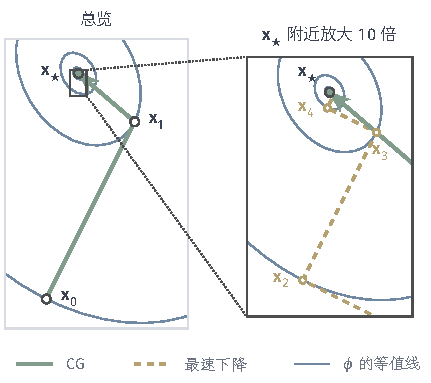
\includegraphics[width=72.873mm]{figures/01-basic-mathematics/03-vectors-matrices-and-multivariate-functions/tikz/c5-cg-steepest-descent-paths/figure.pdf}
  \caption{贯穿例上CG与最速下降的路径。蓝色椭圆是$\phi(\bm x)=\tfrac12\bm x^\top\bm A\bm x-\bm b^\top\bm x$经过最速下降各迭代点的等值线，中心为$\bm x_\star=(1/11,7/11)^\top$。两种方法的第一步都从$\bm x_0=\bm 0$走到$\bm x_1=(1/4,1/2)^\top$；CG的第二个方向与第一个方向$\bm A$共轭，直接指向椭圆中心，最速下降则在$\bm x_\star$附近来回折返（右图为左图小框放大10倍）。}
  \label{fig:ls-cg-steepest-descent-paths}
\end{figure}

\subsection{算法分析}

\paragraph{正确性与收敛速度}
正确性归结为两组关系：残差两两正交，方向两两共轭。由它们可以推出最优性，再由残差多项式得到收敛速度。

\begin{theorem}[CG的最优性与收敛速度]
\label{thm:ls-cg-convergence}
设$\bm A$对称正定，在精确算术下按上述递推计算，且$\bm r_0,\ldots,\bm r_{k-1}$均非零。则$\bm r_0,\ldots,\bm r_k$两两正交，$\bm p_0,\ldots,\bm p_{k-1}$两两关于$\bm A$共轭，$\bm x_k$是$\lVert\bm x-\bm x_\star\rVert_{\bm A}$在$\bm x_0+\mathcal K_k$上的唯一最小点，并且
\begin{equation}
 \lVert\bm x_k-\bm x_\star\rVert_{\bm A}\le2\Bigl(\frac{\sqrt\kappa-1}{\sqrt\kappa+1}\Bigr)^k\lVert\bm x_0-\bm x_\star\rVert_{\bm A},
 \label{eq:ls-cg-convergence-bound}
\end{equation}
其中$\kappa=\kappa_2(\bm A)$。CG至多$d$步得到精确解。
\end{theorem}

\begin{proof}
证明分三步：先证正交与共轭关系，再由它们推出最优性，最后估计收敛速度。

\emph{正交与共轭关系。}对$k$归纳证明：$\bm r_0,\ldots,\bm r_k$两两正交，$\bm p_0,\ldots,\bm p_k$两两共轭，且两组向量都张成$\mathcal K_{k+1}$。$k=0$时显然。设结论对$k$成立，先证$\bm r_{k+1}\perp\mathcal K_{k+1}$。由$\bm p_k=\bm r_k+\beta_{k-1}\bm p_{k-1}$及$\bm r_k\perp\bm p_{k-1}$，
\[
 \bm p_k^\top\bm r_k=\bm r_k^\top\bm r_k ,
\]
于是由步长~\eqref{eq:ls-cg-step}与残差更新~\eqref{eq:ls-cg-update}，
\[
 \bm p_k^\top\bm r_{k+1}=\bm p_k^\top\bm r_k-\alpha_k\bm p_k^\top\bm A\bm p_k=0 .
\]
对$i<k$，由归纳假设中的共轭性，
\[
 \bm p_i^\top\bm r_{k+1}=\bm p_i^\top\bm r_k-\alpha_k\bm p_i^\top\bm A\bm p_k=0 .
\]
$\bm p_0,\ldots,\bm p_k$张成$\mathcal K_{k+1}$，所以$\bm r_{k+1}\perp\mathcal K_{k+1}$，特别地与$\bm r_0,\ldots,\bm r_k$都正交。

再证$\bm p_{k+1}$与此前的方向共轭。对$i<k$，$\bm A\bm p_i\in\mathcal K_{i+2}\subseteq\mathcal K_{k+1}$，故$\bm r_{k+1}^\top\bm A\bm p_i=0$，从而
\[
 \bm p_{k+1}^\top\bm A\bm p_i=\bm r_{k+1}^\top\bm A\bm p_i+\beta_k\bm p_k^\top\bm A\bm p_i=0 .
\]
对$i=k$，由残差更新得$\bm A\bm p_k=(\bm r_k-\bm r_{k+1})/\alpha_k$，再用$\bm r_{k+1}\perp\bm r_k$与式~\eqref{eq:ls-cg-step}、\eqref{eq:ls-cg-beta}，
\[
 \bm r_{k+1}^\top\bm A\bm p_k=-\frac{\bm r_{k+1}^\top\bm r_{k+1}}{\alpha_k}=-\beta_k\,\bm p_k^\top\bm A\bm p_k ,
\]
恰被$\beta_k\bm p_k^\top\bm A\bm p_k$抵消，所以$\bm p_{k+1}^\top\bm A\bm p_k=0$。最后$\bm r_{k+1},\bm p_{k+1}\in\mathcal K_{k+2}$；若$\bm r_{k+1}\ne\bm 0$，两两正交的非零残差线性无关，两组向量都张成$\mathcal K_{k+2}$。

\emph{最优性。}记$\bm e_k=\bm x_k-\bm x_\star$，则$\bm A\bm e_k=-\bm r_k$，且由上一步$\bm r_k\perp\mathcal K_k$。对任意$\bm z\in\mathcal K_k$，
\[
 \lVert\bm e_k+\bm z\rVert_{\bm A}^2
 =\lVert\bm e_k\rVert_{\bm A}^2+2\bm z^\top\bm A\bm e_k+\lVert\bm z\rVert_{\bm A}^2
 =\lVert\bm e_k\rVert_{\bm A}^2+\lVert\bm z\rVert_{\bm A}^2 ,
\]
所以$\bm x_k$是$\bm x_0+\mathcal K_k$上的唯一最小点。$\mathbb R^d$中两两正交的非零向量至多$d$个，故至多$d$步出现零残差。

\emph{收敛速度。}按式~\eqref{eq:ls-krylov-residual-polynomial}的推导，$\bm x_0+\mathcal K_k$中候选的误差为$p(\bm A)\bm e_0$，其中$p\in\mathcal P_k$。由谱定理（定理~\ref{thm:ls-real-symmetric-spectral}）取标准正交特征向量展开$\bm e_0=\sum_ic_i\bm u_i$，得
\[
 \lVert p(\bm A)\bm e_0\rVert_{\bm A}^2=\sum_i\lambda_i\,p(\lambda_i)^2c_i^2\le\max_i p(\lambda_i)^2\,\lVert\bm e_0\rVert_{\bm A}^2 .
\]
由最优性，$\lVert\bm e_k\rVert_{\bm A}$不超过任一$p\in\mathcal P_k$给出的上界，只需构造一个在特征值上很小的$p$。取Chebyshev多项式$T_k$，它由$T_k(\cos\theta)=\cos k\theta$确定，在$[-1,1]$上$\lvert T_k\rvert\le1$；对$x>1$，
\[
 T_k(x)=\tfrac12\bigl[(x+\sqrt{x^2-1})^k+(x-\sqrt{x^2-1})^k\bigr],
\]
因为两边满足同一递推$T_{j+1}=2xT_j-T_{j-1}$和相同初值。令
\[
 \ell(t)=\frac{\lambda_{\max}+\lambda_{\min}-2t}{\lambda_{\max}-\lambda_{\min}},
\]
它把$[\lambda_{\min},\lambda_{\max}]$映到$[-1,1]$，且$\ell(0)=(\kappa+1)/(\kappa-1)$。取
\[
 p(t)=\frac{T_k(\ell(t))}{T_k(\ell(0))}\in\mathcal P_k ,
\]
则在各特征值处$\lvert p\rvert\le1/T_k(\ell(0))$。直接计算，$x=\ell(0)$时$x+\sqrt{x^2-1}=(\sqrt\kappa+1)/(\sqrt\kappa-1)$，于是
\[
 T_k(\ell(0))\ge\frac12\Bigl(\frac{\sqrt\kappa+1}{\sqrt\kappa-1}\Bigr)^k ,
\]
即得所述界。$\kappa=1$时$\bm A$是单位矩阵的倍数，一步得解。
\end{proof}

这个界只依赖两端特征值，误差缩小到给定比例所需的步数约与$\sqrt\kappa$成正比。它控制的是误差的$\bm A$范数，欧氏残差$\lVert\bm r_k\rVert_2$不必每步下降。

\paragraph{数值敏感度}
浮点计算中正交与共轭关系逐步受损，定理的有限步结论不能直接移用，实际计算不承诺恰好$d$步结束；递推残差也会偏离真实残差，所以宣布达到要求前按公共准则用$\bm b-\bm A\bm x_k$复核。

\paragraph{计算代价}
每轮核心递推需要一次$\bm A$乘向量、两次内积和三次向量更新。除矩阵外只保存$\bm x,\bm r,\bm p,\bm q$四个向量，存储不随步数增长；复核真实残差所需的矩阵乘向量另计。
